\documentclass[11pt]{article}

\usepackage{fullpage}
\usepackage{amsmath,amssymb,amsthm,amsfonts,latexsym,bbm,xspace,graphicx,float,mathtools,
verbatim, xcolor} 
\PassOptionsToPackage{hyphens}{url}\usepackage{hyperref}
\newcommand{\new}[1]{\textcolor{red}{#1}}
%\usepackage{psfig}
\usepackage{pgfplots}

\newcommand{\future}[1]{\textcolor{red}{#1}}

\newcommand{\hP}{\hat P}
\newcommand{\hp}{\hat p}

\newcommand{\Dk}{\Delta_k}
\newcommand{\Px}{P(x)}
\newcommand{\Qx}{Q(x)}
\newcommand{\Nx}{N_x}

\newcommand{\Py}{P(y)}
\newcommand{\Qy}{Q(y)}
\newcommand{\Pml}{P_{ML}}
\newcommand{\Pmlx}{\Pml(x)}
\newcommand{\Pbeta}{P_{\beta}}
\newcommand{\Pbetax}{\Pbeta(x)}


\newcommand{\dTV}[2]{d_{TV} (#1,#2)}
\newcommand{\dKL}[2]{D(#1||#2)}
\newcommand{\chisq}[2]{\chi^2(#1,#2)}
\newcommand{\eps}{\varepsilon}

\newcommand{\nPepsp}[1]{n^*(#1, \eps)}
\newcommand{\nPeps}{\nPepsp{\cP}}


\newcommand{\sumX}{\sum_{x\in\cX}}

\newcommand{\Bpr}[1]{Bern(#1)}

\newenvironment{problem}[2][Problem]{\begin{trivlist}
\item[\hskip \labelsep {\bfseries #1}\hskip \labelsep {\bfseries #2.}]}{\end{trivlist}}

% Theorem-like environments

\newtheorem{Theorem}{Theorem}
\newtheorem{Theorem*}{Theorem}

\newtheorem{Claim}[Theorem]{Claim}
\newtheorem{Claim*}[Theorem]{Claim}
\newtheorem{Corollary}[Theorem]{Corollary}
\newtheorem{Conjecture}[Theorem]{Conjecture}
\newtheorem{CounterExample*}{$\overline{\hbox{\bf Example}}$}
\newtheorem{Definition}[Theorem]{Definition}
\newtheorem{Example}[Theorem]{Example}
\newtheorem{Example*}[Theorem]{Example}
\newtheorem{Exercise}[Theorem]{Exercise}
\newtheorem{Intuition*}[Theorem]{Intuition}
\newtheorem{Joke*}[Theorem]{Joke}
\newtheorem{Lemma}[Theorem]{Lemma}
\newtheorem{Lemma*}[Theorem]{Lemma}
\newtheorem{Open problem}[Theorem]{Open problem}
\newtheorem{Proposition}[Theorem]{Proposition}
\newtheorem{Property}[Theorem]{Property}
\newtheorem{Question}[Theorem]{Question}
\newtheorem{Question*}[Theorem]{Question}
\newtheorem{Remark}[Theorem]{Remark}
\newtheorem{Result}[Theorem]{Result}
\newtheorem{Fact}[Theorem]{Fact}
\newtheorem{Condition}[Theorem]{Condition}

\newcommand{\ed}{\stackrel{\mathrm{def}}{=}}
%\newcommand{\edef}{\stackrel{\mathrm{def}}{=}}
\def \Paren#1{{\left({#1}\right)}}

\newcommand{\probof}[1]{\Pr\Paren{#1}}


\newtheorem{theorem}{Theorem}
\newtheorem{proposition}[theorem]{Proposition}
\newtheorem{corollary}[theorem]{Corollary}
%\newtheorem*{corollary*}{Corollary}
\newtheorem{assumption}[theorem]{Assumption}
\newtheorem{lemma}[theorem]{Lemma}
%\newtheorem*{lemma*}{Lemma}
\newtheorem{conjecture}[theorem]{Conjecture}
\newtheorem{example}[theorem]{Example}
\newtheorem{definition}[theorem]{Definition}
\newtheorem{claim}[theorem]{Claim}

\newcommand{\Xon}{X_1^n}


\newcommand{\prob}{{\rm Pr}}
\newcommand{\Probof}[1]{\prob\left(#1\right)}



\newcommand{\ignore}[1]{}

% Equation formatting

\newcommand{\spreqn}[1]{{\qquad\text{#1}\qquad}}

% Blackboard fonts
\newcommand{\II}{\mathbb{I}} % Added by Theertha on April 16th 2013.
\newcommand{\EE}{\mathbb{E}}
\newcommand{\CC}{\mathbb{C}}
\newcommand{\NN}{\mathbb{N}}
\newcommand{\QQ}{\mathbb{Q}}
\newcommand{\RR}{\mathbb{R}}
\newcommand{\ZZ}{\mathbb{Z}}
\newcommand{\PP}{\mathbb{P}}

% Number sets

\newcommand{\complex}{\CC}
\newcommand{\integers}{\ZZ}
\newcommand{\naturals}{\NN}
\newcommand{\positives}{\PP}
\newcommand{\rationals}{\QQ}
\newcommand{\reals}{\RR}

\newcommand{\realsge}{{\reals_{\ge}}}
\newcommand{\realsp}{\reals^+}
\newcommand{\integersp}{\integers^+}
\newcommand{\integerss}[1]{\integers_{\ge{#1}}}

% boldface

\def \ba     {{\bf a}}
\def \bx     {{\bf x}}
\def \by     {{\bf y}}

\def \bA     {{\bf A}}
\def \bB     {{\bf B}}
\def \bC     {{\bf C}}
\def \bD     {{\bf D}}
\def \bF     {{\bf F}}
\def \bG     {{\bf G}}
\def \bL     {{\bf L}}
\def \bQ     {{\bf Q}}
\def \bR     {{\bf R}}
\def \bS     {{\bf S}}
\def \bT     {{\bf T}}
\def \bX     {{\bf X}}
\def \bY     {{\bf Y}}
\def \bZ     {{\bf Z}}

% caligraphics

\def \cA     {{\cal A}}
\def \cB     {{\cal B}}
\def \cC     {{\cal C}}
\def \cD     {{\cal D}}
\def \cE     {{\cal E}}
\def \cF     {{\cal F}}
\def \cG     {{\cal G}}
\def \cH     {{\cal H}}
\def \cI     {{\cal I}}
\def \cK     {{\cal K}}
\def \cL     {{\cal L}}
\def \cM     {{\cal M}}
\def \cN     {{\cal N}}
\def \cO     {{\cal O}}
\def \cP     {{\cal P}}
\def \cQ     {{\cal Q}}
\def \cR     {{\cal R}}
\def \cS     {{\cal S}}
\def \cT     {{\cal T}}
\def \cU     {{\cal U}}
\def \cV     {{\cal V}}
\def \cW     {{\cal W}}
\def \cX     {{\cal X}}
\def \cY     {{\cal Y}}
\def \cZ     {{\cal Z}}

% vectors

\def \vct#1{{\overline{#1}}}

\def \vcta  {{\vct a}}
\def \vctb  {{\vct b}}
\def \vctq  {{\vct q}}
\def \vcts  {{\vct s}}
\def \vctu  {{\vct u}}
\def \vctv  {{\vct v}}
\def \vctx  {{\vct x}}
\def \vcty  {{\vct y}}
\def \vctz  {{\vct z}}
\def \vctp  {{\vct p}}

\def \vctV  {{\vct V}}
\def \vctX  {{\vct X}}
\def \vctY  {{\vct Y}}
\def \vctZ  {{\vct Z}}

\def \vctbeta  {{\vct\beta}}



% qed's --  Also consider \qedhere

\def \eqed    {\eqno{\qed}}
\def \rqed    {\hbox{}~\hfill~$\qed$}

% sequences

\def \upto  {{,}\ldots{,}}

\def \zn    {0\upto n}
\def \znmo  {0\upto n-1}
\def \znpo  {0\upto n+1}
\def \ztnmo {0\upto 2^n-1}
\def \ok    {1\upto k}
\def \on    {1\upto n}
\def \onmo  {1\upto n-1}
\def \onpo  {1\upto n+1}

% sets

\def \sets#1{{\{#1\}}}
\def \Sets#1{{\left\{#1\right\}}}

\def \set#1#2{{\sets{{#1}\upto{#2}}}}

\def \setpmo   {\sets{\pm 1}}
\def \setmpo   {\{-1{,}1\}}
\def \setzo    {\{0{,}1\}}
\def \setzn    {\{\zn\}}
\def \setznmo  {\{\znmo\}}
\def \setztnmo {\{\ztnmo\}}
\def \setok    {\{\ok\}}
\def \seton    {\{\on\}}
\def \setonmo  {\{\onmo\}}
\def \setzon   {\setzo^n}
\def \setzos   {\setzo^*}


% Set operations



\def\ignore#1{}

 

\title{Assignment Eight\\ ECE 4200}
\date{}

\begin{document}
\maketitle 

\begin{itemize}
\item
Provide credit to \textbf{any sources} other than the course staff that helped you solve the problems. This includes \textbf{all students} you talked to regarding the problems. 	
\item
You can look up definitions/basics online (e.g., wikipedia, stack-exchange, etc)
\item
{\bf The due date is 11/13/2020, 23.59.59 eastern time}. 
\item
Submission rules are the same as previous assignments.
\end{itemize}



%\begin{problem}{1. (10 points)}
%Suppose $A$ is a real symmetric matrix. 
%\begin{enumerate}
%\item 
%Show that all eigenvalues of $A$ are real. 
%\item
%Suppose $\overrightarrow x$, and $\overrightarrow y$ are two eigenvectors of $A$ with eigenvalues $\lambda_1$, and $\lambda_2$ respectively. Suppose $\lambda_1\ne\lambda_2$, then show that $\overrightarrow{x}\cdot \overrightarrow{y}= \overrightarrow{x}^T\overrightarrow{y}=0$. This shows that eigenvectors with different eigenvalues are orthogonal to each other.
%\item
%Find the eigenvectors and eigenvalues of the matrix
%\[
%\begin{bmatrix}
%    3 & 2 & 4 \\
%    2 & 0 & 2  \\
%    4 & 2 & 3
%\end{bmatrix}.
%\]
%\end{enumerate}
%\end{problem}

% Find the eigenvectors and eigenvalues of the matrix
% \[
% \begin{bmatrix}
%     8 & -1 & 2 \\
%     -1 & -2 & 2  \\
%     2 & 2 & -6
% \end{bmatrix}.
% \]
% \end{enumerate}
% \end{problem}

\begin{problem}{1. (15 points)}
Consider one layer of a ReLU network. The feature vector is $d$ dimensional $\overrightarrow x$. The linear transformation is a $m\times d$ dimensional matrix $W$. The output of the ReLU network is a $m$ dimensional vector $y$ given by $\max\{\mathbf{0}, W\overrightarrow x\}$. This is a component-wise max function. 
\begin{itemize}
	\item Suppose $\overrightarrow x$ is fixed, and all its entries are non-zero.
	\item Suppose the entries in $W$ are all independent, and distributed accoding to a Gaussian distribution with mean 0, and standard deviation 1 (a $N(0,1)$ distribution).
\end{itemize} 
\begin{itemize}
	\item [1.] Show that the expected number of non-zero entries in the output is $m/2$.  
	\item [2.] Suppose $\|\overrightarrow x\|_2^2 = \sigma^2$, what is the distribution of each entry in $Wx$ (the output before applying ReLU function)?
	\item [3.] What is the mean of each entry in $y$ (after ReLU function)?
\end{itemize}

\end{problem}
%
%\begin{problem}{2. (10 points)}
%	Suppose at the $i$th layer of the neural network, you have $n_i$ neurons $\mathbf{z}^i = (z^i_1, z^i_2, z^i_3, ..., z^i_{n_i})$. Assume they are all independent and each of them has variance $\sigma^2$. Suppose at the next layer, before activation, we have $n_{i+1}$ neurons $\mathbf{z}^{i+1} = (z^{i+1}_1, z^{i+1}_2, z^{i+1}_3, ..., z^{i+1}_{n_i})$. Let $W^{n_{i+1} \times n_i}$ be the weight matrix, then we have:
%	\[
%		\mathbf{z}^{i+1}  = W \mathbf{z}^i
%	\]
%	
%	Let $W_k$ be the $k$th row of matrix $W$, show that for all $k \in \{1,2,...,n_{i+1}\}$:
%	\[
%		Var(z^{i+1}_k) = |W_k|_2^2 \sigma^2
%	\]
%	where $|W_k|_2^2 = \sum_{j=1}^{n_i} W(k,j)^2$.
%\end{problem}

\begin{problem}{2. (10 points)}
Consider the setting as in the previous problem, with $m=2$, and $d=2$. Let
\[
W = \begin{bmatrix}
    1 & 2 \\
    -2 & 3   \\
\end{bmatrix},
\overrightarrow x = \begin{bmatrix}
2\\
-3
\end{bmatrix}.
\]
%Consider the function $L = \max\{\sigma(W \overrightarrow x)\}$. Please draw the computational graph for this function, and compute the gradients (which will be Jacobians at some nodes!).
Consider the function $L = \max\Big \{\sigma \small(W_{(1)} \overrightarrow x\small), \sigma \small(W_{(2)} \overrightarrow x \small)\Big\}$, where $\sigma$ is the Sigmoid function and $W_{(i)}$ denotes the $i$th row of $W$. Please draw the computational graph for this function, and compute the gradients (which will be Jacobians at some nodes!).
\end{problem}


\begin{problem}{3. (10 points)}
	Given inputs $z_1, z_2\in \RR$, the softmax function is the following:
	\[
		\hat{y} = \frac{e^{z_1}}{e^{z_1} + e^{z_2}}.
	\]
	Let $y \in \{0, 1\}$, then define the cross-entropy loss between $y$ and $\hat{y}$ be
	\[
		L(y, \hat{y}) = -y\log(\hat{y}) - (1-y)\log(1-\hat{y}).
	\]
	Prove that:
	\[
		\frac{\partial L(y,\hat{y})}{\partial z_1} = \hat{y} - y, \frac{\partial L(y,\hat{y})}{\partial z_2} = y - \hat{y}.
	\]
\end{problem}

\begin{problem}{4. (15 points)}
	Consider datapoints in Figure~\ref{fig-NN}: $(-2, 0), 
	(2 ,0)$ are crosses, and $(0, 2), (0,-2)$ are circles. Let the crosses be labeled $+1$, and the circles be labeled $-1$. 
	\begin{figure}[htb]
		\centering
		\begin{tikzpicture}[scale=0.8]
		\begin{axis}[
		axis lines=middle,
		xmin=-5, xmax=5,
		ymin=-5, ymax=5,
		xtick=, ytick=
		]
		\addplot [only marks, mark=x, mark options={red}] table {
			-2 0
			2 0
		};
		\addplot [only marks, mark=o, mark options={blue}] table {
			0 2
			0 -2
		};
		\end{axis}
		\end{tikzpicture}
		\caption{Neural Networks}
		\label{fig-NN}
	\end{figure}
	In this problem the goal is to design a neural network with no error on this dataset. 
	
	To make things simple, consider the following generalization. We first append a $+1$ to each input and form a new dataset as follows: $(-2, 0, 1), 
	(2 ,0, 1)$ are labeled $+1$, and $(0, 2,1), (0,-2,1)$ are labeled $-1$. Note that the last feature is redundant.
	
	We consider the following basic units for our neural networks: Linear transformation followed by hard thresholding. Each unit has three parameters $w_1, w_2, w_3$. The output of the unit is the sign of the inner product of the parameters with the input. 
	
	\begin{figure}[h]
		\centering
		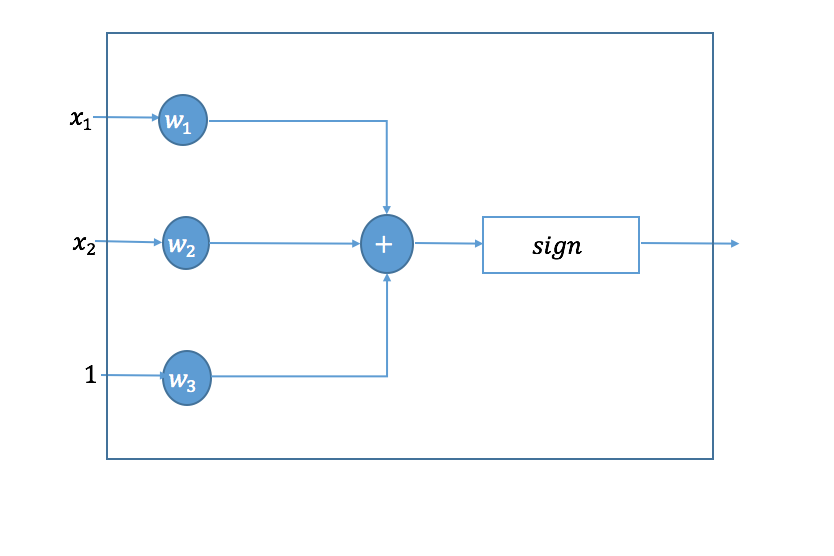
\includegraphics[width=0.5\linewidth]{figo.png}
		\label{fig1}
	\end{figure}
	
	\begin{itemize}
		\item[1.] Design a neural network with these units that make no error on the datapoints above. (Hint: You can take two units in the first layer, and one in the output layer, a total of three units). 
		\item[2.] 
		Show that if you design a neural network with ONLY one such unit, then the points cannot be all classified correctly.
	\end{itemize}
\end{problem}

\begin{problem}{5. (40 points)} See attached notebook for details.
%In this problem, you will implement a 2-layer (1 hidden layer) neural network using \textbf{only Numpy} libraries and no other external libraries like sklearn or pytorch. We will use the wdbc dataset for this problem. Please download it again if you haven't. \par
%Please use the following architecture  
%\begin{itemize}
%\item Number of hidden neurons : 20 
%\item Activation function after first hidden layer : ReLU, sigmoid 
%\item Softmax layer after output layer (this is needed because we are using the cross-entropy loss)
%\item Loss function : cross-entropy loss 
%\item Weight updates using Gradient Descent with learning rates $1,0.1,0.01,0.001$ 
%\end{itemize} 
%Please do the following : 
%\begin{itemize}
%\item  Plot the training error and test error as a function of the number of epochs (max number of epochs = 10000) for each activation function (ReLU, sigmoid). After examining the plots, which activation function would you prefer ? 
%\item For both the activation functions, plot the training error and test error while varying the learning rate as $\dfrac{0.1}{\sqrt{n}}$, where $n$ is the current epoch. Do you see an improvement in the convergence rate on the training error compared to the fixed learning rate ?
%\end{itemize}
%Please refer to the skeleton provided in the jupyter notebook. Note that this skeleton is merely a guideline to get you started. You don't necessarily need to follow the skeleton.
\end{problem}

\end{document}